\documentclass[11pt,dvipdfmx,a4paper]{jsarticle}

\usepackage{amsmath,amssymb}
\usepackage{bm}
\usepackage[dvipdfmx]{graphicx}
\usepackage{physics} % http://mirrors.ibiblio.org/CTAN/macros/latex/contrib/physics/physics.pdf
\usepackage{siunitx} %SI単位を楽に出力
\usepackage{mathtools} %環境の追加
% \usepackage{circuitikz} %電気回路をtex中で書く
% \usepackage{caption} %番号なしキャプションを書く
% \usepackage{cancel} %式中に斜線を入れる
% \usepackage{tensor} %テンソルの添え字を書く
% \usepackage{tikz} %図を書く
% \usepackage{ascmac} %四角い枠の中に文章を書く
% \usepackage{float} %figureで[hbp]オプションを使う
% \usepackage{hyperref}  \usepackage{pxjahyper} %ハイパーリンクをつかう
% \usepackage{tablefootnote} %表中に注釈をいれる
% \usepackage[thicklines]{cancel} %数式中の取り消し線
% \usepackage[version=4]{mhchem} %化学式の入力
\usepackage{pdfpages}
\usepackage{wrapfig} %文章の回り込み
\usepackage[subrefformat=parens]{subcaption} %(a)図のようにすることができるやつ
\usepackage{here}
\usepackage[margin=15mm]{geometry} %余白の削除

\graphicspath{{./image/}}

\begin{document}

%出力したpdfを表紙にするとき
% \includepdf[pages=1,noautoscale=false]{cover.pdf}
% \newpage

%texで表紙を書くとき
\quad\\[35mm]
\centerline{\Huge{\textsf{第 2 回}}}
\quad\\[5mm]
\centerline{\Huge{\textsf{応 用 物 理 学 実 験}}}
\quad\\[5mm]
\begin{table}[h]
	\centering
	\begin{tabular}{| c | c |}
		\hline
		\Huge\textsf{{題目}} & \Huge{\textsf{電子回路}} \rule[-5mm]{0mm}{15mm} \\
		\hline
	\end{tabular}
\end{table}
\quad\\[10mm]
\begin{table}[h]
	\centering
	\begin{tabular}{l l}
		\hline
		\LARGE{\textsf{氏\qquad 名}} & \LARGE{\textsf{: 西原 翔}} \rule[0mm]{0mm}{6mm} \\
		\hline
		\LARGE{\textsf{学  籍  番  号}} & \LARGE{\textsf{: 1522068}} \rule[0mm]{0mm}{6mm} \\
		\LARGE{\textsf{学部学科学年}} & \LARGE{\textsf{: 理学部第一部応用物理学科3年}}\\
		\hline
	\end{tabular}
\end{table}
\quad\\[10mm]
\centerline{\LARGE{\textsf{共同実験者:1522064 中井空弥}}}\\[2mm]
\quad\\[10mm]
\centerline{\LARGE{\textsf{提出年月日:2024年05月30日}}}\\[2mm]
\centerline{\LARGE{\textsf{実験実施日:2024年05月10日}}}\\[2mm]
\centerline{\LARGE{\textsf{\qquad\qquad\quad\;2024年05月17日}}}
\quad\\[10mm]
\centerline{\LARGE{\textsf{東 京 理 科 大 学 理 学 部 第 1 部}}}\\[2mm]
\centerline{\LARGE{\textsf{応 用 物 理 学 教 室}}}

\thispagestyle{empty}
\clearpage
\addtocounter{page}{-1}
\newpage

% \twocolumn
\section{目的}
オペアンプは電子回路で用いられる素子の一つで、
二つの入力電圧を受け取りその差を大きな倍率で出力する。
この性質により、入力信号の増幅とフィルタリングであったり、加算、減算、微分といった計算、
出力をまた入力に戻してフィードバックループを作って制御に用いられるなど重要な役割を果たしている。

オペアンプには回路の解析が簡単になるよい性質があり、その性質を用いてこの素子を用いた回路設計を行っていくことが多い。
しかしこれは一種の近似であるため、この手法が成り立たない領域がある。

この実験ではオペアンプを活用した回路である反転増幅回路、ボルテージ・フォロワ回路、2 次のローパスフィルタ回路の 3 つ回路の振舞いを実際に測定した。

\section{原理}
\subsection{オペアンプ}
% オペアンプの歴史を電子回路の本から引っ張ってくる

オペアンプには五つの端子があり模式図と、
今回の実験で実際に使う素子 LM741 は図\ref{fig:no1} のようになっている。
2 番ピンの反転入力端子の電圧を \(V_{-}\), 3 番ピンの非反転入力端子の電圧を\(V_{+}\), 6 番ピンの出力端子の電圧を \(V_o\) とする。
電圧増幅度を \(\mu\simeq 10^5\) としたとき、これらの間には
\begin{equation}
	V_o = \mu (V_{+} - V_{-})
\end{equation}
となっている。
電圧を増幅するためのエネルギー減として
出力電圧は 4 番ピンの負電源と 7 番ピンの正電源をつなぐ必要がある。
これらの端子を超える電圧を出力することはできない。(課題1)
このような状態を出力飽和という。

出力端子を入力端子につなげることを考える。
このとき入力電圧と出力電圧はほぼ同じオーダーとなるため、
大きな電圧増幅度との積をとる\(V_{+} - V_{-}\)この値は 電圧増幅度の逆数のオーダーでなければならない。
\(\mu\simeq10^5\) であるため、\(V_{+}=V_{-}\) と言ってもよい。
つまり反転入力端子と非反転入力端子が短絡されているとみなせる状態となっている。
このように反転入力端子と非反転入力端子の電圧を考えるのを仮想短絡と呼ぶ。

また、理想的なオペアンプは入力に関しては電圧だけを見て入力部の回路には干渉せず、
出力は決まった電圧を出すため電流を吸い込むものと考える。
これは入力については電圧計と同様に入力インピーダンスを限りなく大きく、
出力は電圧源と同様に出力インピーダンスは限りなく小さいものとみなす。

この二つの性質はある一定の条件における近似になっているので成り立つときと成り立たないときに気を付けて
回路の設計をしなければならない。
\begin{figure}[H]
	\centering
	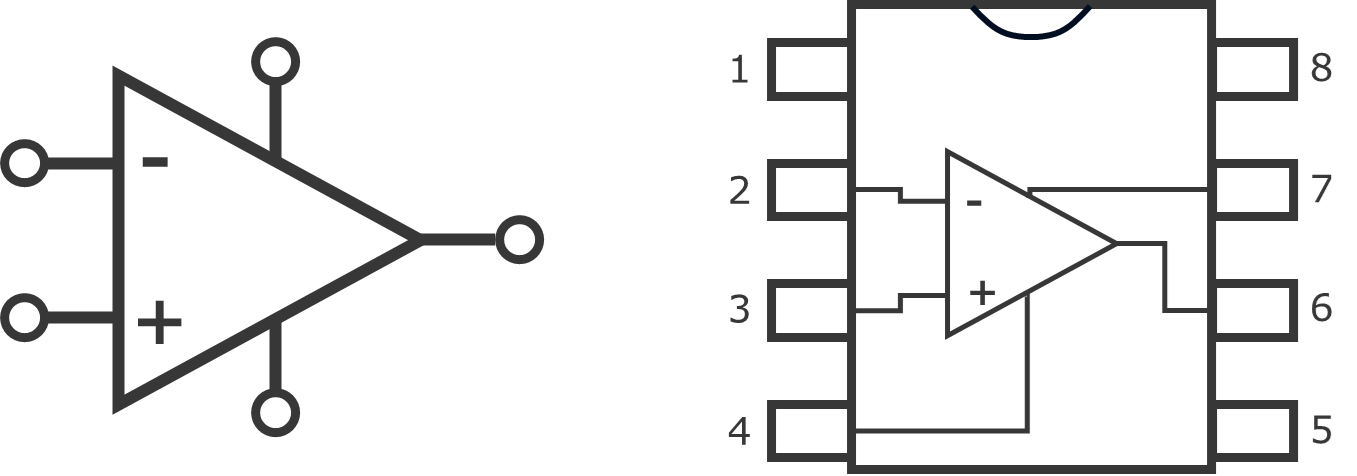
\includegraphics[width = 0.7 \columnwidth]{/fig/OpeAmp.png}
	\caption{オペアンプの回路図と LM741 のピン配置。
	1 番ピンはオフセット調整端子、
	2 番ピンは反転入力端子、
	3 番ピンは非反転入力端子、
	4 番ピンは負側電源端子、
	5 番ピンはオフセット調整端子、
	6 番ピンは出力端子、
	7 番ピンは正側電源端子、
	8 番ピンは不使用というようになっている。}
	\label{fig:no1}
\end{figure}
\newpage

\subsection{反転増幅回路}
入力電圧を逆位相で増幅し出力する回路を反転増幅回路と言い、
オペアンプを使ったものとしては図\ref{fig:no2}がある。
仮想短絡により
\begin{equation}
	V_{-} = 0 \text{ V}
\end{equation}
である。
この回路に入力された電流はオペアンプの入力端子に流れず、\(R_{f}\) にすべて流れる。
そのため\(R_i\) の抵抗に流れる電流と、\(R_f\) の抵抗に流れる電流について等式を立てて整理していくと、
\begin{align}
	\frac{V_i-V_{-}}{R_i} &= \frac{V_{-}-V_o}{R_f}\\
	V_0 &= -\frac{R_f}{R_i} V_i
\end{align}
というようになる。

\subsection{ボルテージ・フォロワ回路回路}
\begin{wrapfigure}{r}[0pt]{0.5\columnwidth}
	\centering
	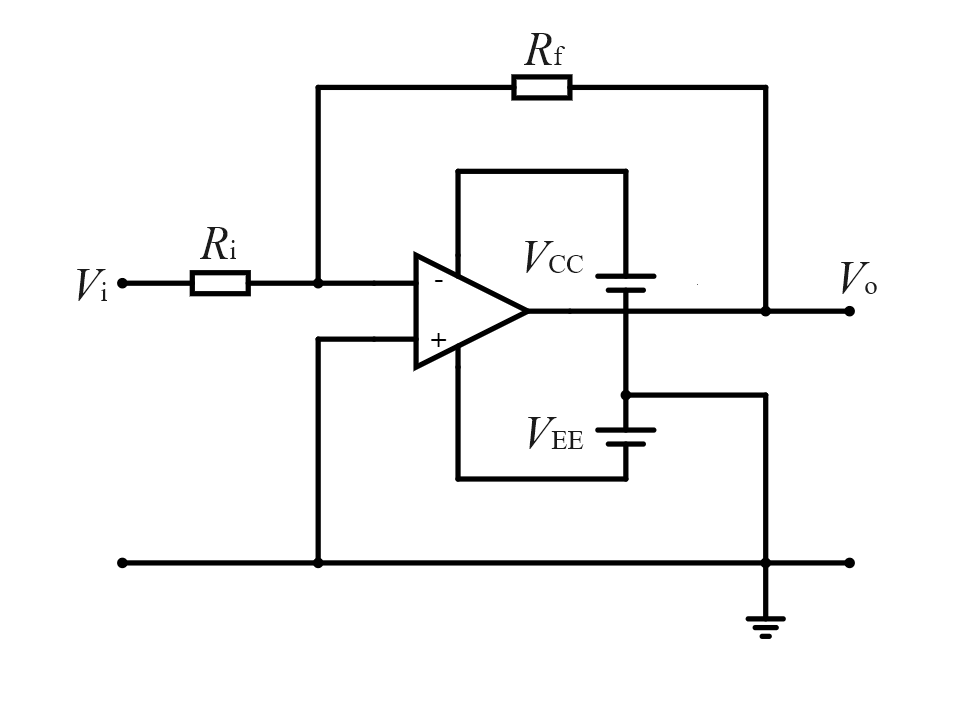
\includegraphics[width = 0.5\columnwidth]{/fig/Invert_Amp_Circuit.png}
	\caption{反転増幅回路の回路図}
	\label{fig:no2}
\end{wrapfigure}
\begin{figure}[b]
	\begin{minipage}[t]{0.49\columnwidth}
		\centering
		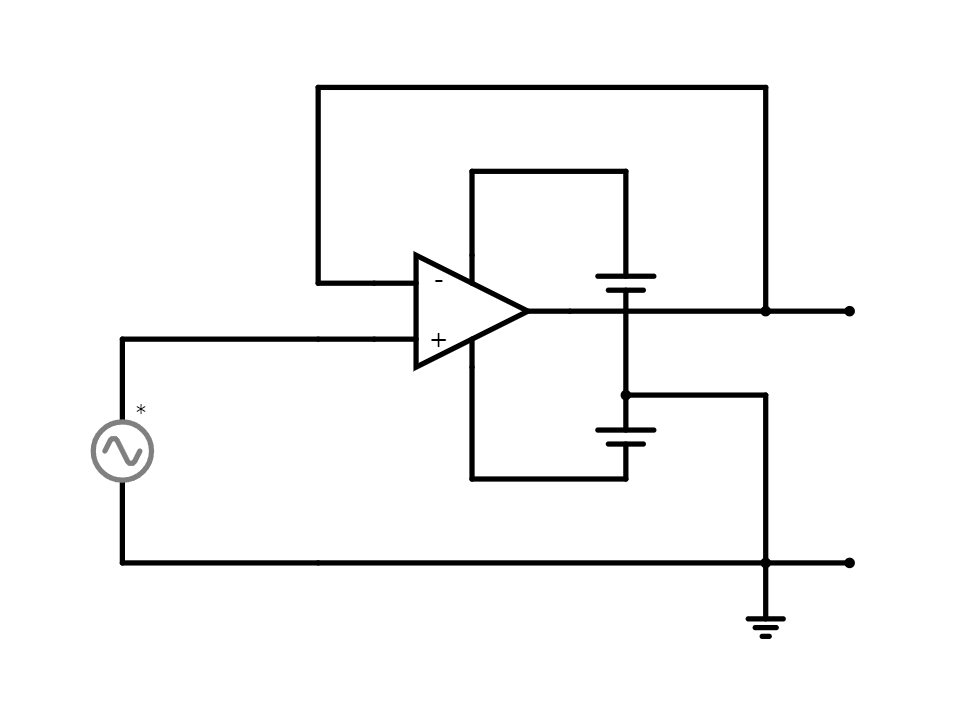
\includegraphics[width = \columnwidth]{/fig/Voltage_Follower_Circuit.png}
		\caption{ボルテージ・フォロワ回路の回路図}
		\label{fig:no3}
	\end{minipage}
	\hfill
	\begin{minipage}[t]{0.49\columnwidth}
		\centering
		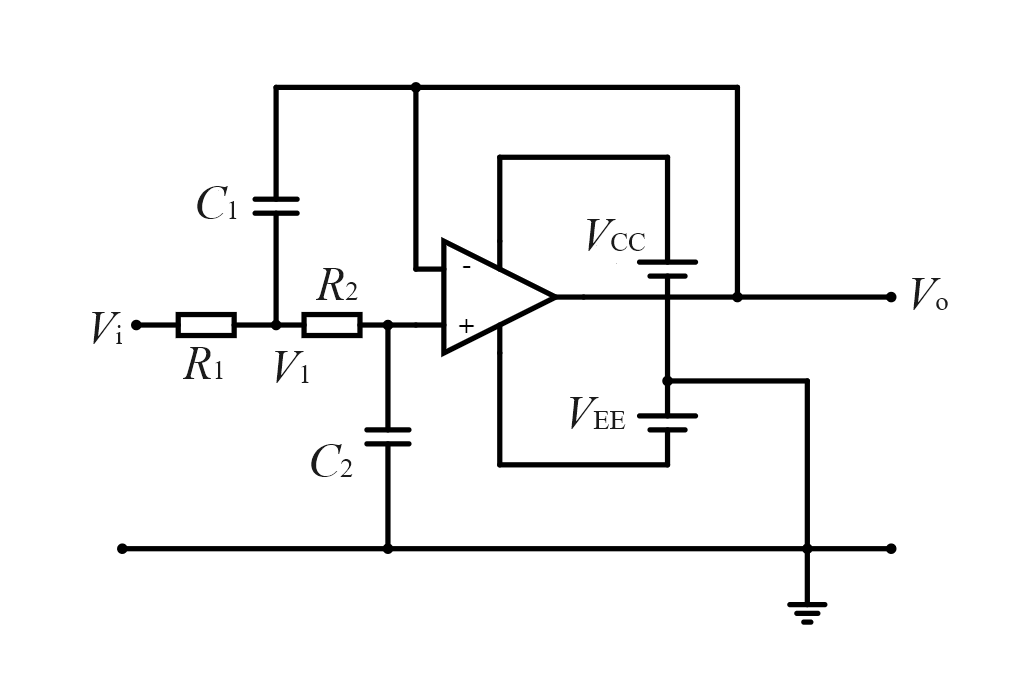
\includegraphics[width = \columnwidth]{/fig/Low_Pass_Filter.png}
		\caption{2次のローパス・フィルタ回路の回路図}
		\label{fig:no4}
	\end{minipage}
\end{figure}
回路を設計する際、入力となる部分の回路と出力となる部分の回路を干渉させたくないことがある。
そういったときに入力には電圧だけを読み取り電流を吸い込まず、
出力では決まった電圧を出力し必要に応じて電流を出すといった回路が求められる。
そういった回路をバッファ回路という。
理想オペアンプは入力は電圧だけ読み取り電流は流さず出力は決まった電圧を出力する素子であるため、
バッファ回路として使われることがある。
図\ref{fig:no3}のように反転入力端子と出力を結びつけると、
非反転入力端子には電流が流れ込まず、
仮想短絡により入力が等倍で出力されていることがわかる。

実際のオペアンプは IC 部分の応答の速さにより入力信号が瞬時に出力されない。
この実験では 2 種類のオペアンプ LM741 と TL071 の応答の様子を確認した。


\subsection{2次のローパス・フィルタ回路}

交流入力があったとき、特定の周波数だけを取り除く回路をフィルタ回路といい、
とくに高周波成分を取り除く回路をローパスフィルタ回路という。
その例が図\ref{fig:no4} である。
これについて解析していく。(課題2)
仮想短絡により
\begin{equation}
	V_{+} = V_{-} = V_o. \label{eq:low-pass-1}
\end{equation}
電圧\(V_1\)と書かれた地点において電流の流出入を考えると
\begin{equation}
	\frac{V_i-V_1}{R_1}+\frac{V_{-}-V_1}{1/sC_1} = \frac{V_1-V_{+}}{R_2} \label{eq:low-pass-2}.
\end{equation}
また電圧\(V_{+}\)と書かれた地点において電流の流出入を考えるとオペアンプには電流が流れ込まないので
\begin{equation}
	\frac{V_1-V_{+}}{R_2} = \frac{V_{+}}{1/sC_2} \label{eq:low-pass-3}
\end{equation}
となる。これらの式を整理してを入力と出力の比である伝達関数\(G(s)\)を求める。
(\ref{eq:low-pass-1}) 式と(\ref{eq:low-pass-3}) 式より
\begin{equation}
	V_1 = V_o \qty(1+sC_2 R_2).
\end{equation}
これを (\ref{eq:low-pass-3})式に入れていくと
\begin{align}
	\frac{V_i-V_1}{R_1}+\frac{V_{o}-V_1}{1/sC_1} &= \frac{V_{o}}{1/sC_2}\\
	V_i &= V_o \biggl\{(C_1C_2R_1R_2)s^2+(R_1+R_2)C_2s+1\biggr\}\\
	G(s) &= \frac{V_o}{V_i} = \frac{\omega_c^2}{s^2+2\zeta\omega_c s+\omega_c^2} \label{eq:low-pass-4}
\end{align}
となる。ここで共振周波数\(\omega_c\) と制動係数\(\zeta\) は次のとおりである。
\begin{align}
	\omega_c &:= \frac{1}{\sqrt{C_1C_2R_1R_2}},\\
	\zeta &:= \frac{1}{2}\sqrt{\frac{C_2}{C_1}}\qty(\sqrt{\frac{R_1}{R_2}}+\sqrt{\frac{R_2}{R_1}}).
\end{align}

\section{実験}
\subsection{反転増幅回路}
図\ref{fig:no2} の反転増幅回路をブレッドボード上に組んでその振る舞いを調べた。
オペアンプは LM741 を使い、オペアンプに \(\pm 15.0 V\) の電圧を供給した。
また抵抗 \(R_f\) は 100 k\si{\ohm} として、\(R_i\) は各測定で切り替えた。
\subsubsection{直流特性}
直流特性を調べるため入力として -10 V から 10 V の電圧をかけたときの
反転入力端子の電圧\(V_{-}\) と出力電圧\(V_{o}\) を
\(R_i =\) 33 k\si{\ohm} のときと
\(R_i =\) 68 k\si{\ohm} のときの両方を測定した。

\subsubsection{交流電圧特性}
交流電流の振幅の入出力特性を調べた。
\(R_i =\) 33 k\si{\ohm} のときと
\(R_i =\) 68 k\si{\ohm} のときそれぞれにおいて、
10 kHz の交流電圧を入力したときに実効値を 0 V から 10 V まで変えたときの出力電圧を測定した。

\subsubsection{交流周波数特性}
\(R_i =\) 33 k\si{\ohm} のときと
\(R_i =\) 15 k\si{\ohm} のときそれぞれにおいて、
実効値 1.0 V の交流電圧の周波数を 100 Hz から 100 kHz まで変化させたときの出力電圧を測定した。

\subsection{ボルテージ・フォロワ回路}
図\ref{fig:no3}のボルテージ・フォロワ回路をブレッドボード上に組んだ。
オペアンプの種類による応答の波形の違いをもとめるためスルーレートという量を使う。
入力信号に対する出力信号の遅れを表す量として矩形波を入れたときの出力の立ち上がりの傾きをスルーレートと呼び単位は V/s である。
この数字が大きければ大きいほど信号に対する応答が早いものと言える。
この実験では LM741 と TL071 のオペアンプの応答の違いを見た。
使用した矩形波は 10 kHz で peak-to-peak が 10V であった。

\subsection{2 次のローパス・フィルタ回路}
図\ref{fig:no4}の 2 次のローパス・フィルタ回路をブレッドボード上に組み、
伝達関数の制動係数\(\zeta\)を変えたときにていったときのゲインと位相の周波数依存性を 10 Hz から 20 kHz まで測定した。
また 300 Hz で peak-to-peak が 1V の矩形波を入力したときの波形
このとき位相はオシロスコープについている機能を用いて測定した。
使用したオペアンプは LM741 で、\(\pm 15.0 V\) の電圧を供給した。
制動係数を変えるのに使った抵抗とコンデンサのインピーダンスは表\ref{table:no1}のようになっている。
\begin{table}[H]
	\centering
	\caption{2次のローパス・フィルタ回路(図\ref{fig:no4})に使用した抵抗とコンデンサのパラメータ}
	\label{table:no1}
	\begin{tabular}[t]{cccccc}
		\hline
		\(R_1\) (k\si{\ohm}) & \(R_2\) (k\si{\ohm}) & \(C_1\) (nF) & \(C_2\) (nF) & \(\omega_c\) (rad/s) & \(\zeta\)\\
		24 & 10 & 10 & 10 & 6455 & 1.10\\
		24 & 10 & 22 & 47 & 6348 & 0.51\\
		24 & 10 & 47 & 22 & 634 & 0.24\\
		\hline
	\end{tabular}
\end{table}

\section{結果}
\subsection{反転増幅回路}
\subsubsection{直流特性}
反転増幅回路の直流特性の測定結果は図\ref{graph:no1}のようになった。
\(R_i\) が 33 k\si{\ohm} の回路は
入力電圧が -4.01 V から 4.00 V の間において、回路の解析通りに
出力は位相が反転して、倍率が\(R_i/R_f = 3.09\) で動作しているのがわかる。
また反転入力端子の電位は仮想短絡により 0 V になっているというのがわかる。
一方この範囲を超えると、 -13.6 V 程度の一定の電圧を出力するようになった。
これはオペアンプにかけた電源電圧 \(\pm\)15 V であるので飽和出力になったと考えられる。
またこのとき、反転入力端子の電圧が 0 V から変化し始めた。

\(R_i\) が 16 k\si{\ohm} の回路ではこの測定範囲においては
回路の解析通りに動作していることがわかる。
ただ、10 V 付近の反転入力端子のの測定値をみると上昇し始めているのが読み取れる。
これは 33 k\si{\ohm} の回路での振る舞いと照らし合わせると、
これ以上の電圧を入力に入れると出力飽和になると予想される。

\subsubsection{交流電圧特性}
反転増幅回路の交流電圧特性の測定結果は図\ref{graph:no2}のようになった。
\(R_i\) が 33 k\si{\ohm} の回路、\(R_i\) が 16 k\si{\ohm} の回路ともに
出力の実効値が 10.3 V より小さいときには回路の解析通りに振舞うことがわかる。
実行値を実際の振幅に直すと\(\pm 14.6\) V となる。
これもやはり、解析通りに作動しないのは飽和出力状態になっているのが原因だとわかる。
また入力周波数を十分上げると出力は三角波のようになった。(図\ref{graph:noA})

\subsubsection{交流周波数特性}
反転増幅回路の直流特性の測定結果は図\ref{graph:no3}のようになった。
これを見ると両方の回路において 10 kHz より低い周波数においては、
解析通りのゲインとなっているのがわかる。
一方周波数が 10 kHz より大きいときにおいては 20 dB/dec でゲインが減少していることがわかる。
このゲインの減少の傾きから反転増幅回路は 1 次のローパス・フィルタ回路のような振る舞いをしていることがわかる。

\begin{figure}[H]
	\centering
	\begin{minipage}[t]{0.49\columnwidth}
		\centering
		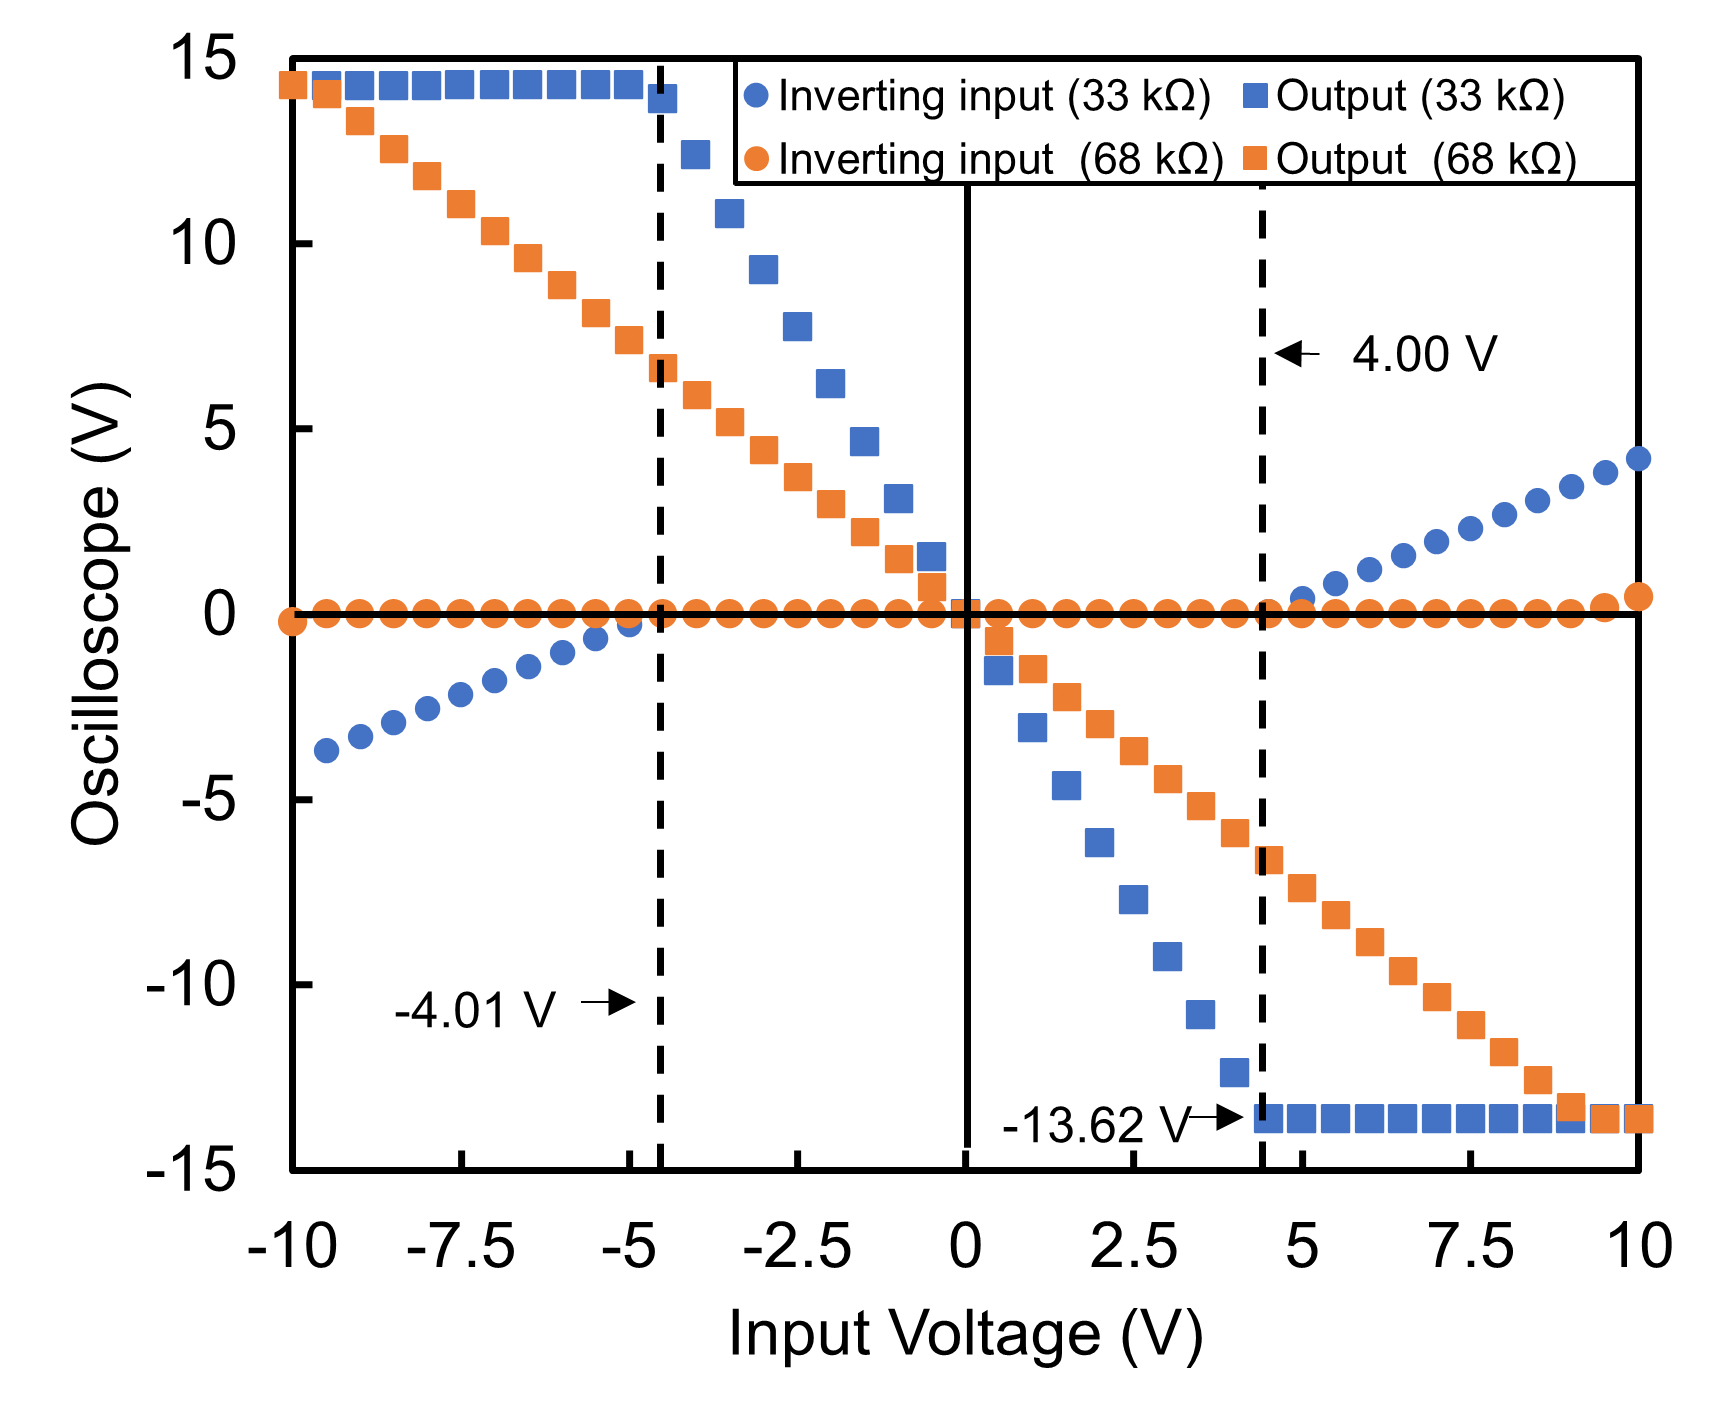
\includegraphics[width=\columnwidth]{/graph/fig1.png}
		\subcaption{直流特性}
		\label{graph:no1}
	\end{minipage}
	\hfill
	\begin{minipage}[t]{0.49\columnwidth}
		\centering
		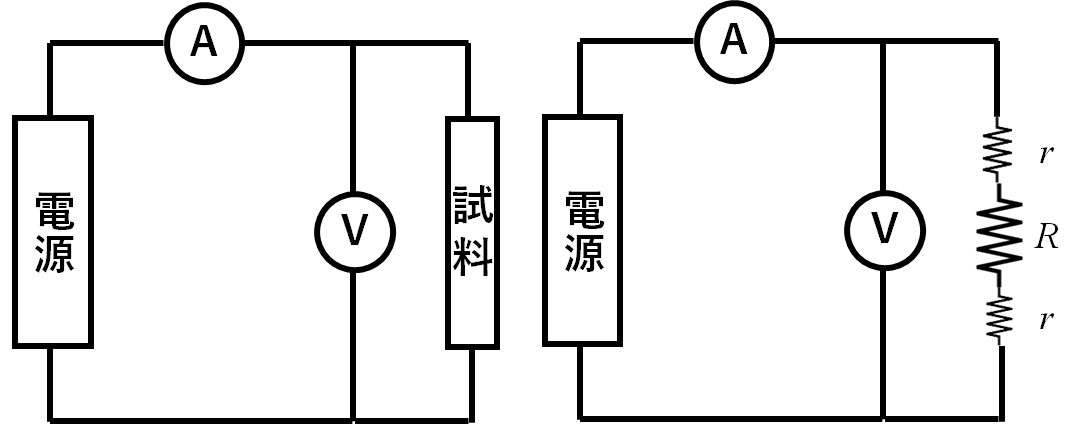
\includegraphics[width=\columnwidth]{/graph/fig2.png}
		\subcaption{交流電圧特性}
		\label{graph:no2}
	\end{minipage}\\
	\begin{minipage}[t]{0.49\columnwidth}
		\centering
		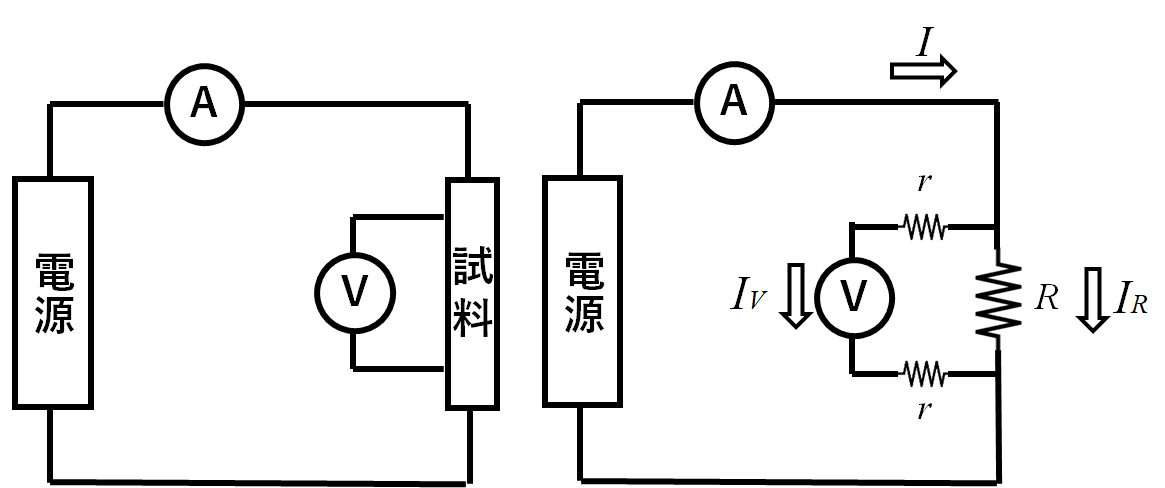
\includegraphics[width=\columnwidth]{/graph/fig3.png}
		\subcaption{交流周波数特性}
		\label{graph:no3}
	\end{minipage}
	\hfill
	\begin{minipage}[t]{0.49\columnwidth}
		\centering
		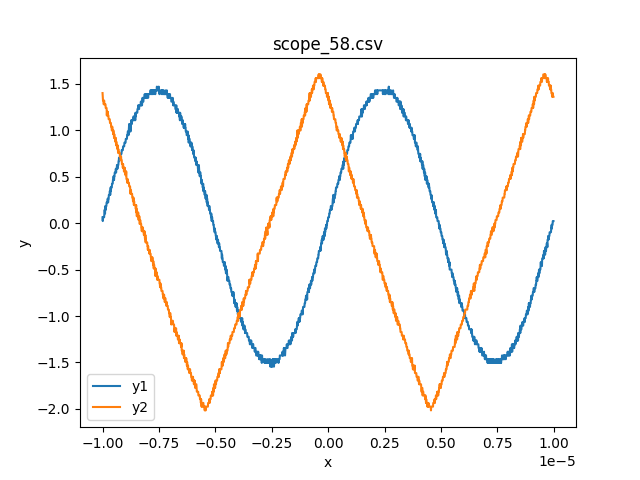
\includegraphics[width=\columnwidth]{/graph/scope_58.csv.png}
		\subcaption{入力周波数が10 kHz における入出力波形。
		横軸が時間(s) で縦軸が電圧 (V), 入力が青色で出力が赤色。}
		\label{graph:noA}
	\end{minipage}
	\caption{LM741 を使用した反転増幅回路の特性の測定結果。
	このときの\(R_f\) は 100 k\si{\ohm} である。}
\end{figure}

\subsection{ボルテージ・フォロワ回路}
ボルテージ・フォロワ回路の矩形波に対する応答は
オペアンプに LM741 を使ったものは図\ref{graph:no6},
オペアンプに TL071 を使ったものは図\ref{graph:no7} のようになった。
このグラフよりスルーレートを求めると
LM741 では 1 V/\si{\micro s},
TL071 では 10 V/\si{\micro s} となった。
\begin{figure}[H]
	\centering
	\begin{minipage}[t]{0.49\columnwidth}
		\centering
		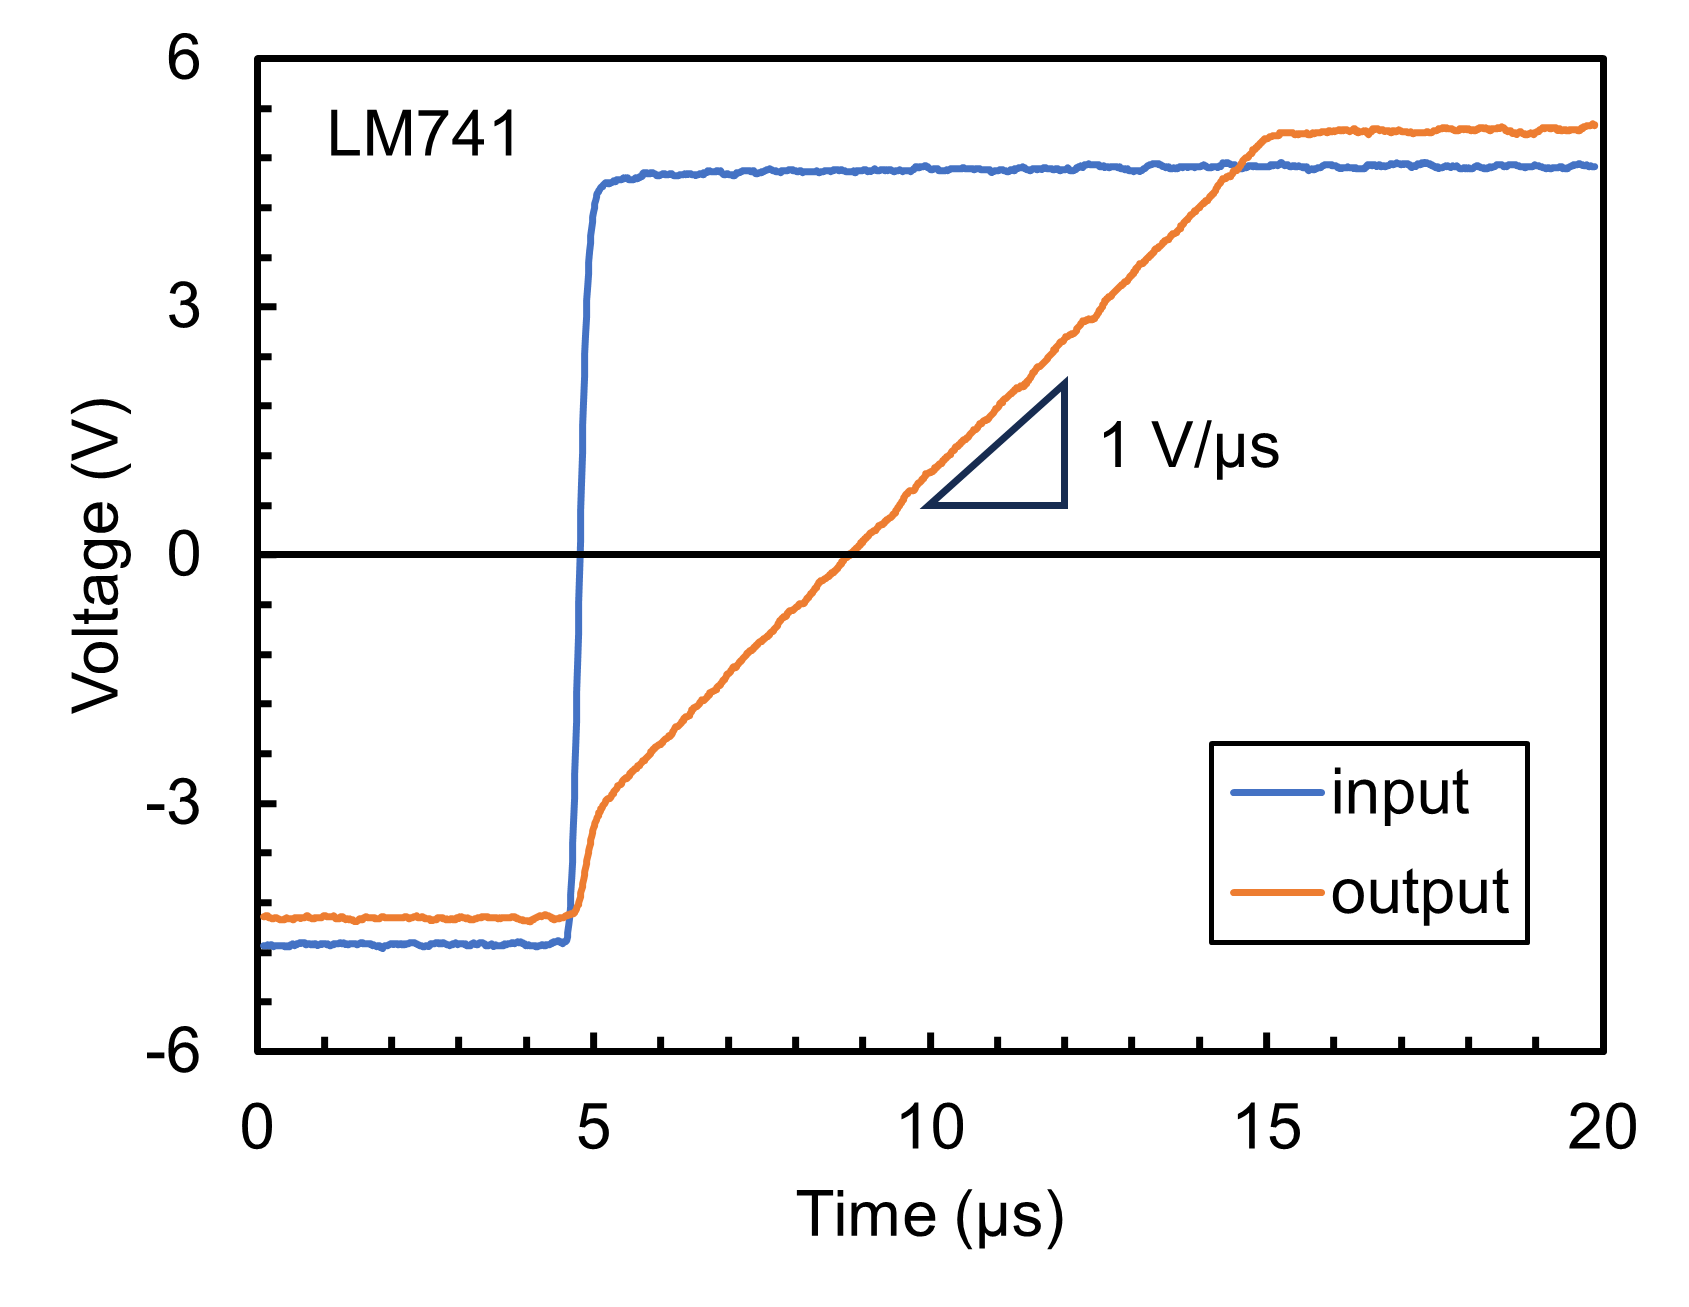
\includegraphics[width=\columnwidth]{/graph/fig6.png}
		\subcaption{LM741}
		\label{graph:no6}
	\end{minipage}
	\hfill
	\begin{minipage}[t]{0.49\columnwidth}
		\centering
		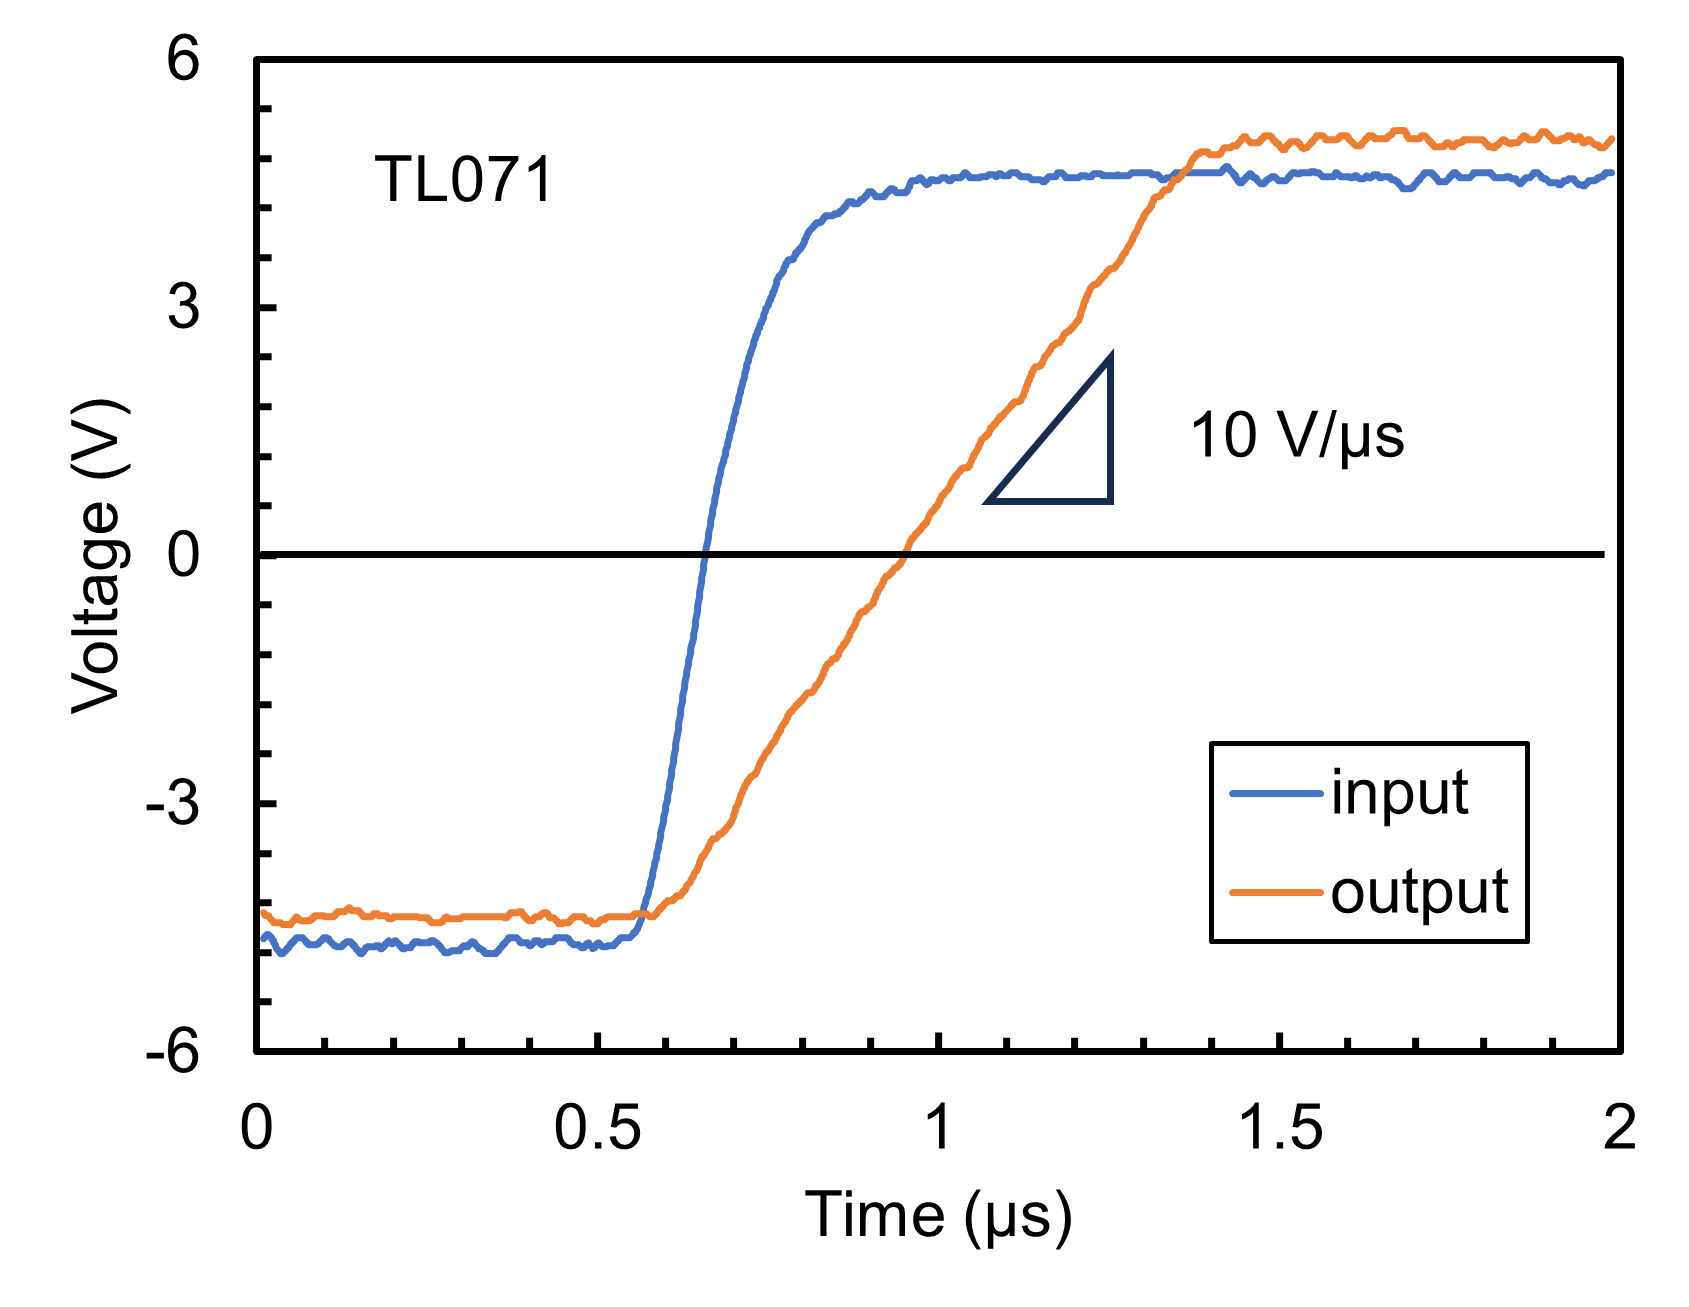
\includegraphics[width=\columnwidth]{/graph/fig7.png}
		\subcaption{TL071}
		\label{graph:no7}
	\end{minipage}
	\caption{ボルテージフォロワ回路に peak to peak : 10 V, 周波数 10 kHz の矩形波を入力したときの出力の様子。
	測定した電圧は移動平均線をとってノイズを減らしてある。}
\end{figure}

\subsection{2 次のローパス・フィルタ回路}
2 次のローパス・フィルタ回路のゲインの周波数特性は図\ref{graph:no4},
入力と出力の位相差の周波数特性は図\ref{graph:no5}のようになった。
\(\zeta = 1.10\) のように制動係数が大きいときには共振周波数 \(\omega_c\) より低い周波数の時点で減衰が始まっていて、
\(\zeta = 0.24\) のように制動係数が小さいときには共振周波数 \(\omega_c\) 付近で増幅を起こす振る舞いが確認できる。
これは共振周波数以下の周波数成分は残し、それ以上の周波数成分を取り除くというローパス・フィルタとしては不適切なゲイン特性になっている。
また(\ref{eq:low-pass-4})式とのずれがゲイン・位相ともに見られないことから、回路の寄生成分が見られないものとわかる。
これはR, L, C の素子から作るローパス・フィルタ回路との違いにもなっている。
また、2 次のローパス・フィルタであるため、1 次のローパス・フィルタ(図\ref{graph:no3}) よりも減衰する速さが速いことから
ローパスフィルタとしての性能こちらの方がよいのがわかる。

矩形波をローパス・フィルタに通したときの出力は図\ref{graph:no9}のようになった。
\begin{figure}[H]
	\centering
	\begin{minipage}[t]{0.49\columnwidth}
		\centering
		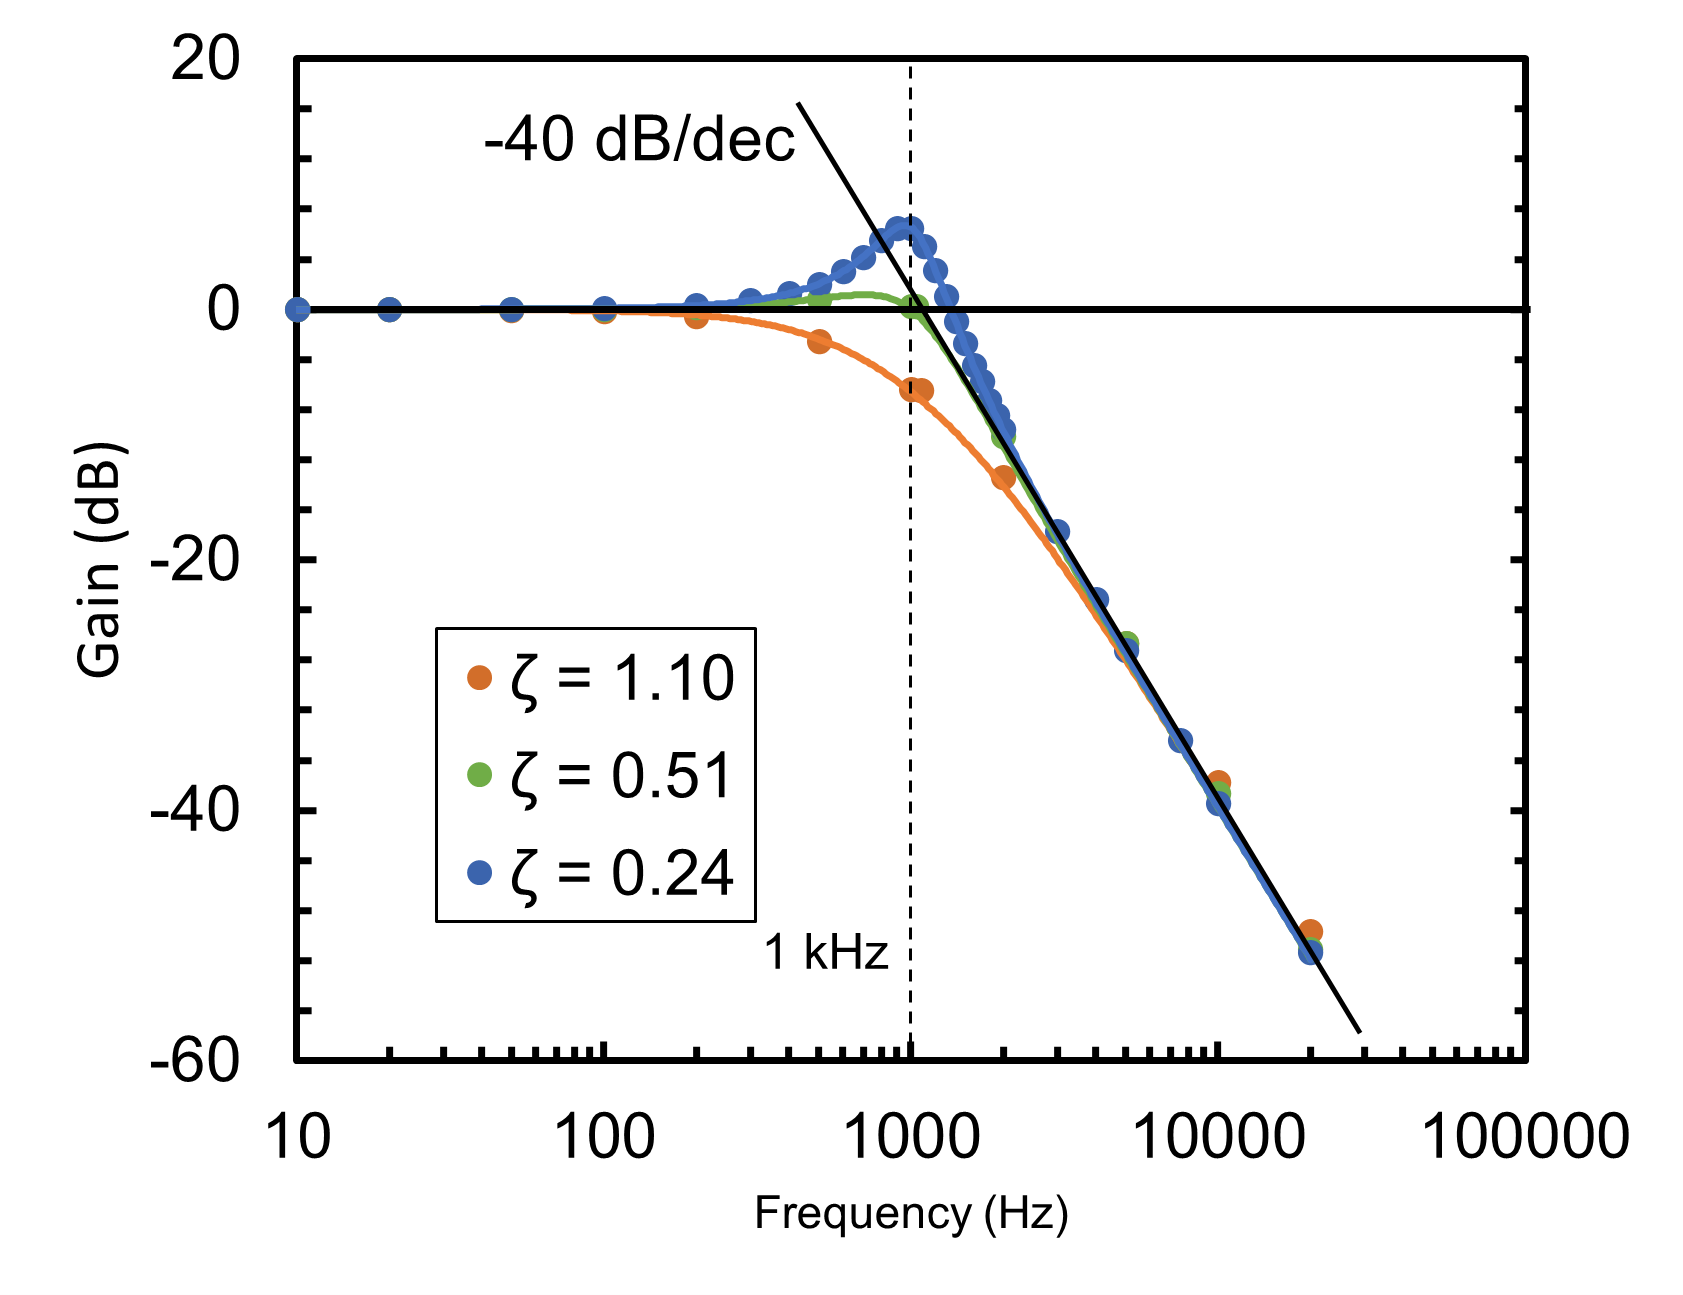
\includegraphics[width=\columnwidth]{/graph/fig4.png}
		\subcaption{ゲイン}
		\label{graph:no4}
	\end{minipage}
	\hfill
	\begin{minipage}[t]{0.49\columnwidth}
		\centering
		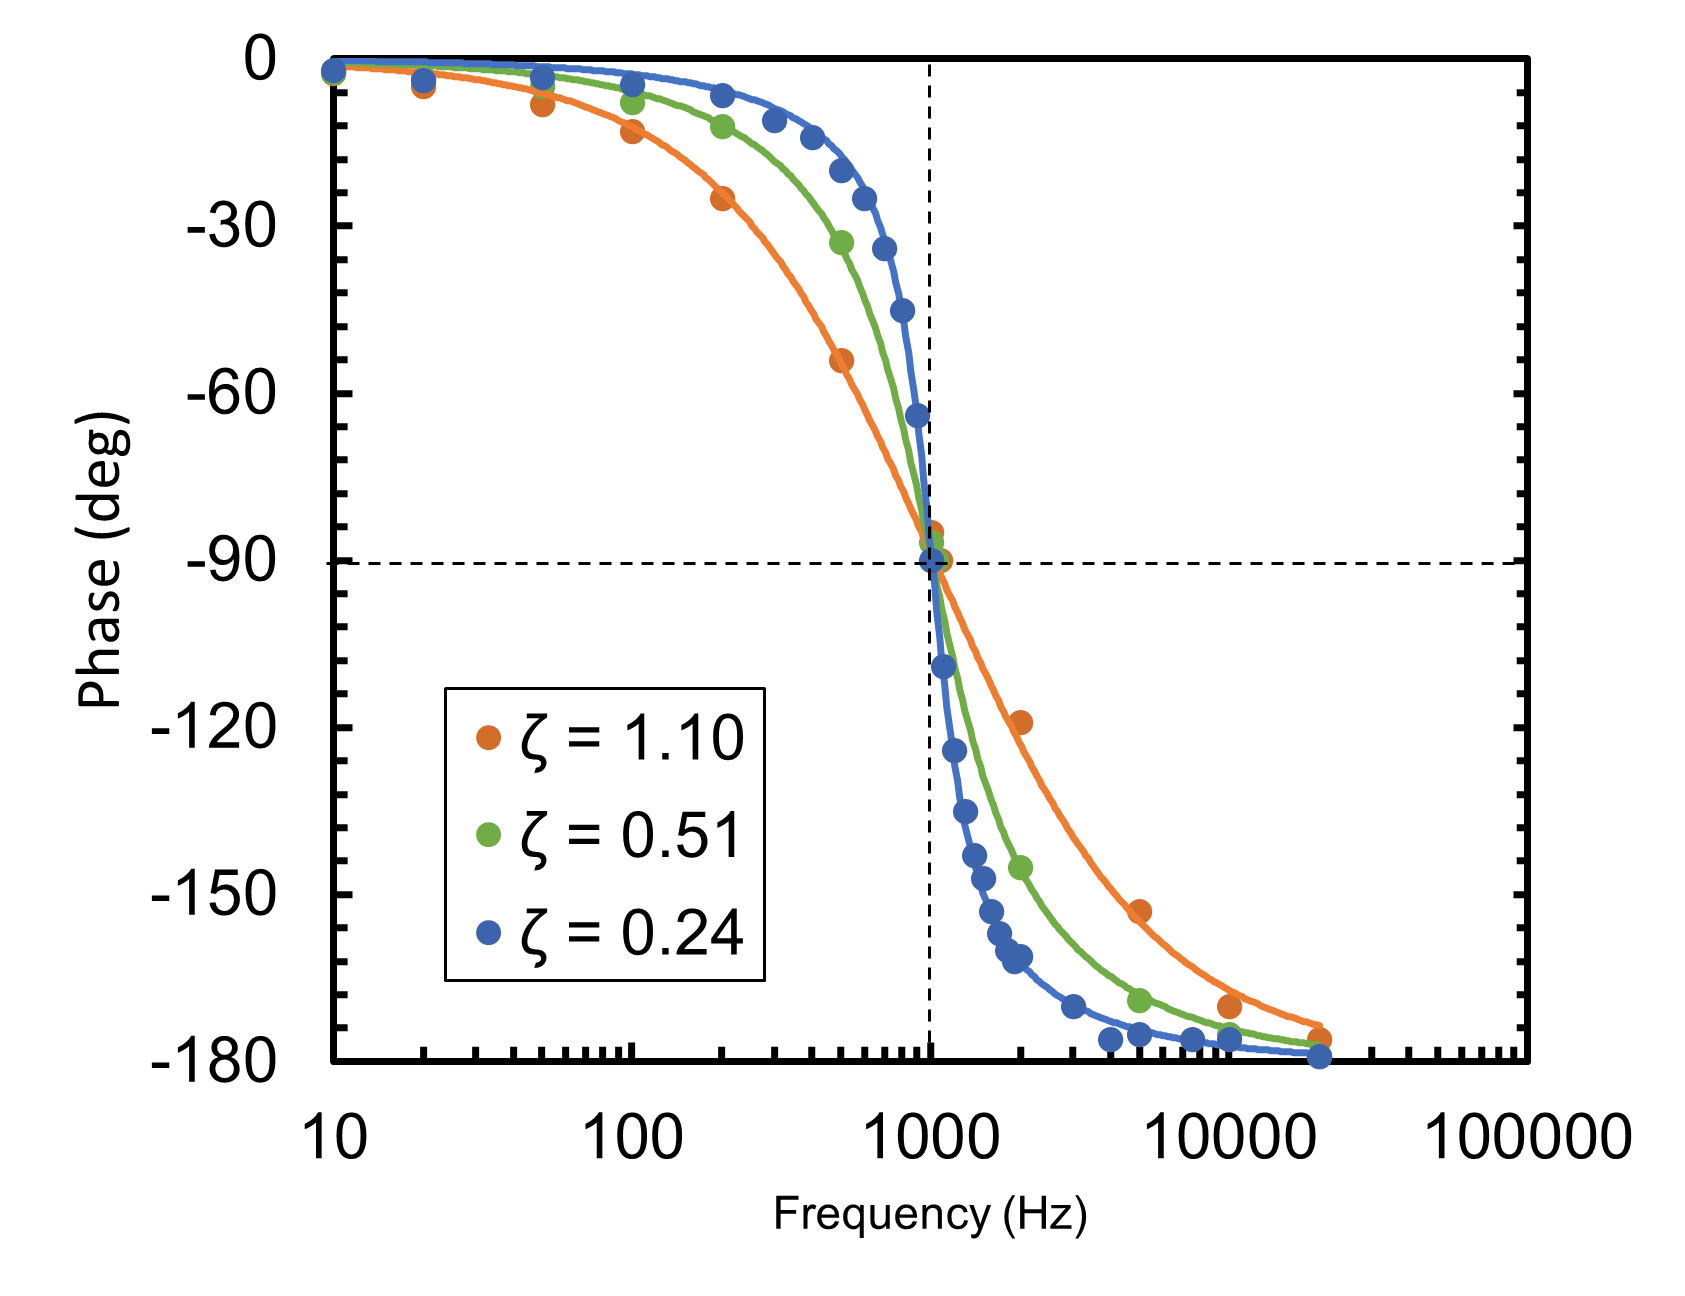
\includegraphics[width=\columnwidth]{/graph/fig5.png}
		\subcaption{位相}
		\label{graph:no5}
	\end{minipage}
	\caption{LM741 を使った 2 次のローパス・フィルタ回路周波数特性の測定結果。
	実線は(\ref{eq:low-pass-4})式に共振周波数 \(\omega_c\) と 制動係数\(\zeta\)の値を入れて得られたもの。}
\end{figure}

\begin{figure}[H]
	\centering
	\begin{minipage}[t]{0.55\columnwidth}
		\centering
		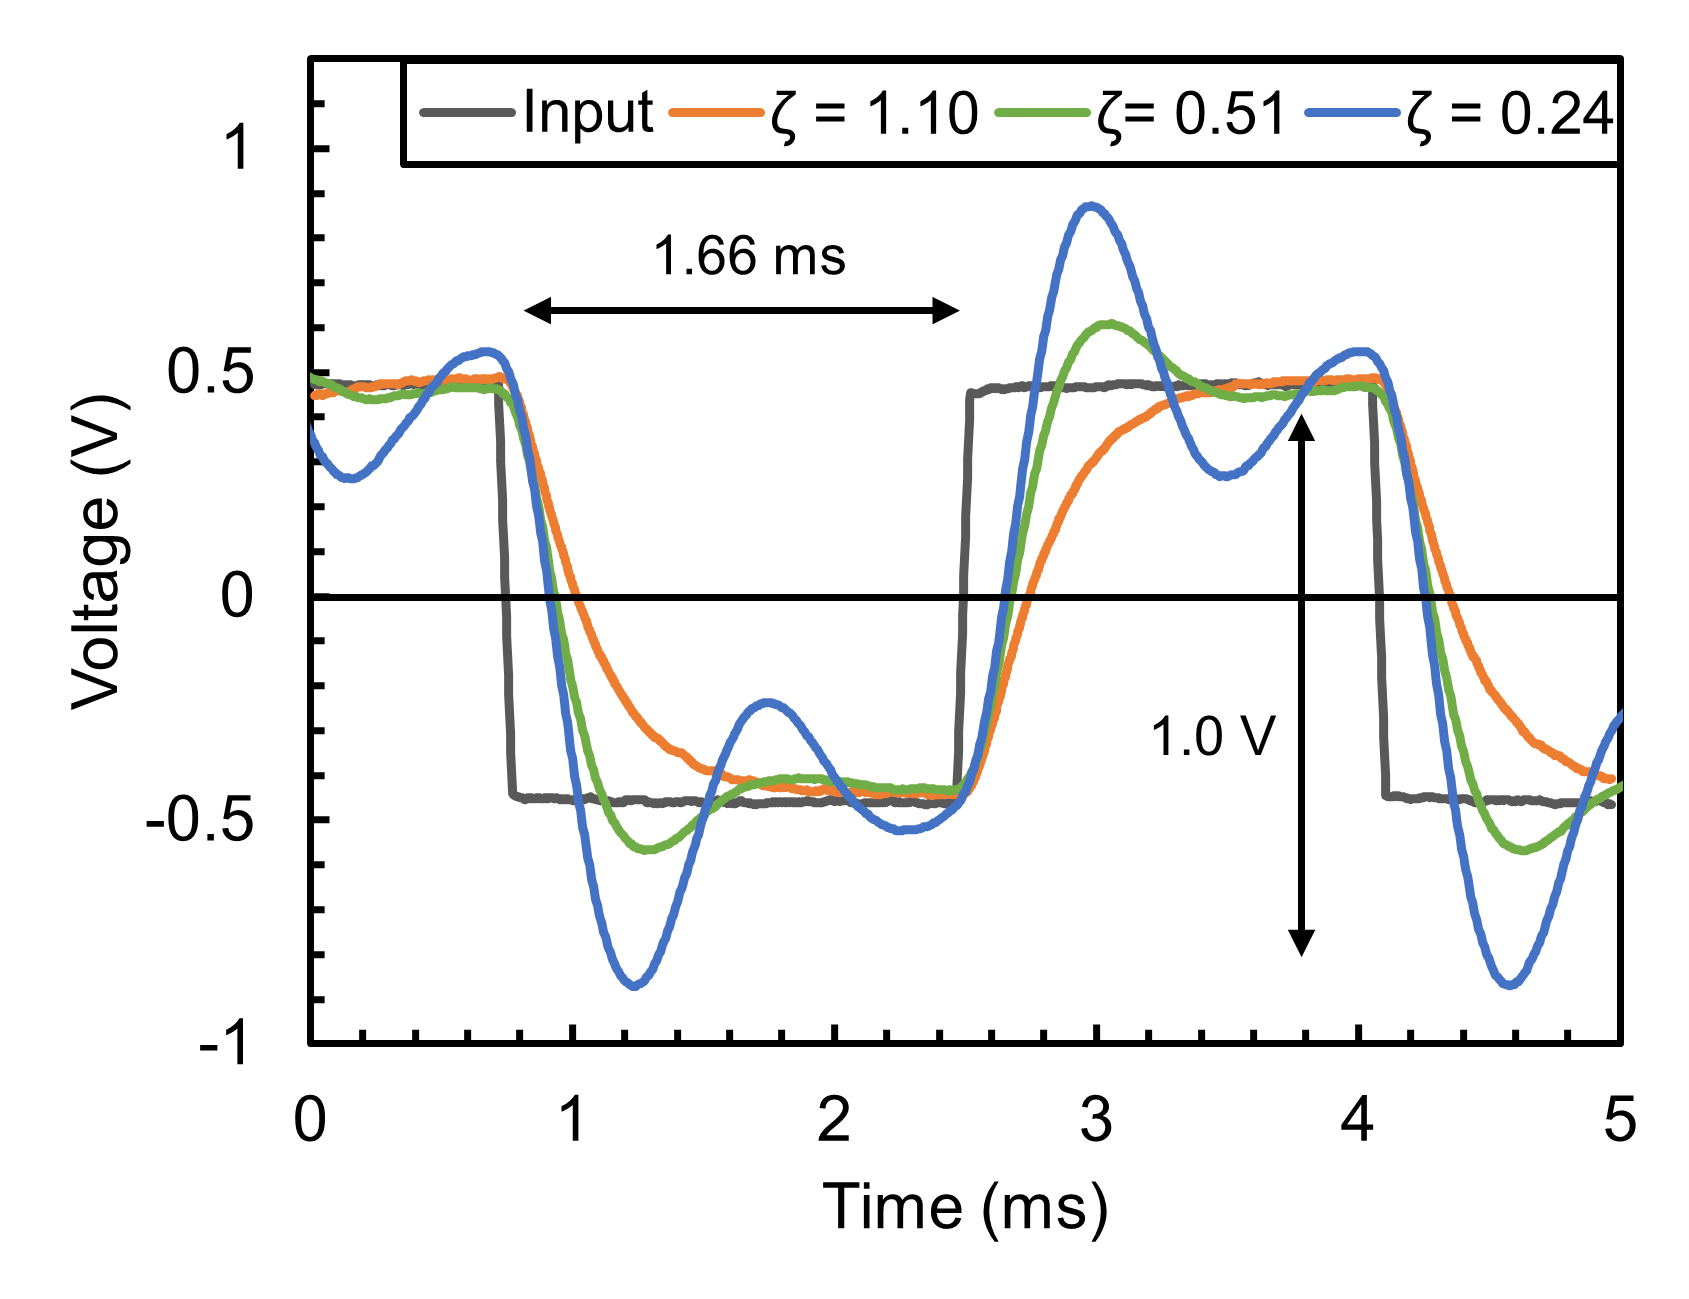
\includegraphics[width=\columnwidth]{/graph/fig9.png}
		\caption{peak-to-peak が 1V, 周波数が 300 Hz の矩形波を入力したときの出力の様子。
		移動平均でノイズを除去してある。}
		\label{graph:no9}
	\end{minipage}
	\hfill
	\begin{minipage}[t]{0.42\columnwidth}
		\centering
		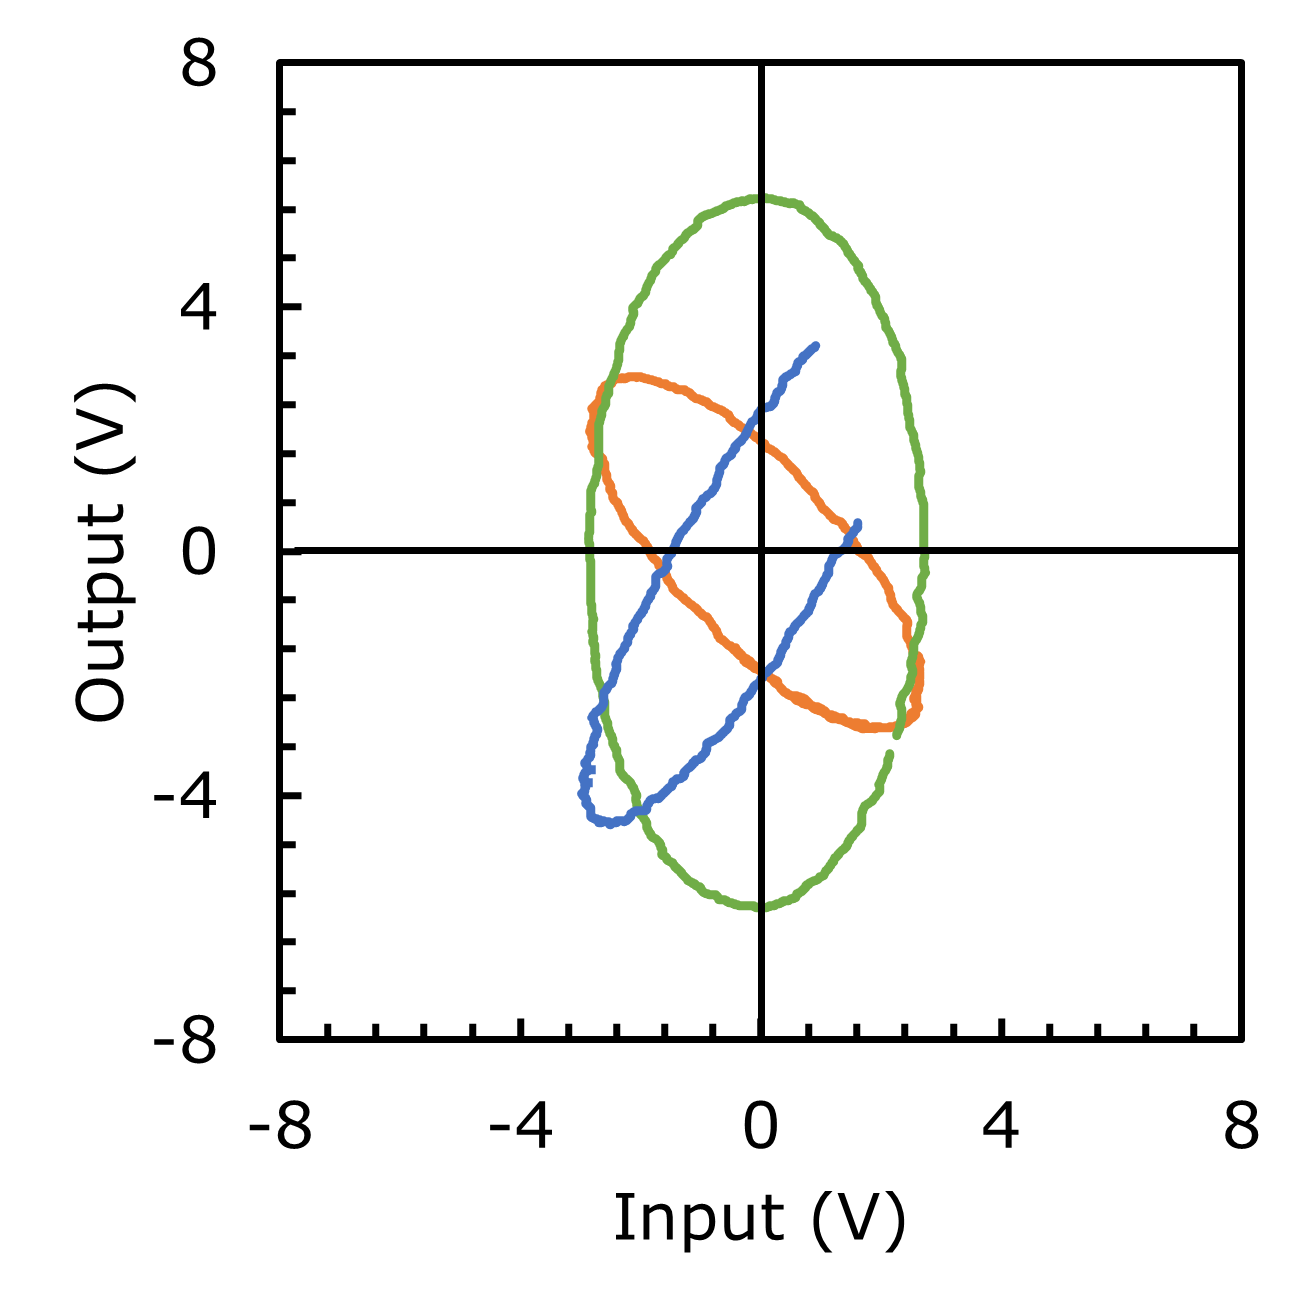
\includegraphics[width=\columnwidth]{/graph/fig8.png}
		\caption{2 次のローパス・フィルタ回路の入力と出力をオシロスコープの X-Y モードで出力した様子。}
		\label{graph:no8}
	\end{minipage}
\end{figure}

\section{考察}
\subsection{反転増幅回路における高周波での出力波形が三角波になる要因}
図\ref{graph:noA}のグラフを見ると三角波になっているのがわかる。
ただ周波数特性のグラフ(図\ref{graph:no3})をみると周波数がカットされるような振動数ではない。
そのため 1 次のローパス・フィルタとして反転増幅回路が働いたのが原因ではない。

これはオペアンプの応答が追い付いていないことが原因のように見える。

\section{結論}


さらなる検討の例\cite{huga}も存在するが、この説明では不十分とする場合もある\cite{hoge}。

\bibliographystyle{junsrt}
\bibliography{reference}

\end{document}